\documentclass[12pt]{report} % ---- COMPILE WITH XeLaTeX for Unicode!!! ----
\usepackage[a4paper, top=1in, bottom=1in, left=1.5in, right=1in]{geometry} % Set margins
\usepackage{setspace} % allows \doublespacing & \singlespacing
\usepackage{parskip} % enables non-indented paragraphs with a blank line
\UseRawInputEncoding

\usepackage[export]{adjustbox}
\usepackage{listings}
\usepackage{xcolor}
% enables graphics, all figures and images should be in the /figures/ folder:
\usepackage{graphicx}

\def\changemargin#1#2{\list{}{\rightmargin#2\leftmargin#1}\item[]}
\let\endchangemargin=\endlist 
% enhanced maths symbols and syntax:
\usepackage{amsmath}
\usepackage{amssymb}
\usepackage{amsthm} % if you need mathematical definitions and theorems

\usepackage[ruled]{algorithm2e} % allow for algorithms in pseudocode
\usepackage{listings} % allow for source code algorithms/listings
\lstset{basicstyle=\footnotesize, frame=single, numbers=left} % customise listing style

% Customise chapter headings so they are of the format: 1. Introduction
\usepackage{titlesec}
\titleformat{\chapter}[block]
  {\normalfont\huge\bfseries}{\thechapter.}{1em}{\Huge}
\titlespacing*{\chapter}{0pt}{-20pt}{20pt}

% Setup bibliography - add file to project named bibliography.bib
% can create this from Zotero, Mendeley, refworks, etc
\usepackage{natbib}
\bibliographystyle{agsm}
\setcitestyle{authoryear,open={(},close={)}, aysep={,}}

\usepackage{hyperref} % add links to document



% Colored Python listing from https://www.overleaf.com/learn/latex/Code_listing
\definecolor{codegreen}{rgb}{0,0.6,0}
\definecolor{codegray}{rgb}{0.5,0.5,0.5}
\definecolor{codepurple}{rgb}{0.58,0,0.82}
\definecolor{backcolour}{rgb}{0.95,0.95,0.92}
 
\lstdefinestyle{mystyle}{
    backgroundcolor=\color{backcolour},   
    commentstyle=\color{codegreen},
    keywordstyle=\color{magenta},
    numberstyle=\tiny\color{codegray},
    stringstyle=\color{codepurple},
    basicstyle=\ttfamily\footnotesize,
    breakatwhitespace=false,         
    breaklines=true,                 
    captionpos=b,                    
    keepspaces=true,                 
    numbers=left,                    
    numbersep=5pt,                  
    showspaces=false,                
    showstringspaces=false,
    showtabs=false,                  
    tabsize=2
}
\lstset{style=mystyle}



\doublespacing
\begin{document}

% 

 \begin{titlepage}
 \topskip0pt
\vspace*{\fill}

    \begin{center}
        
\includegraphics[width=0.6\textwidth]{images/logo.png}
        
        \huge
        \textbf{Self Organizing Maps}
        \vspace{0.5cm}
 
        \Large
        
        \textbf{ \href{mailto:am05427@st.habib.edu.pk}{{Akeel Ather Medina - am05427}}}
        
        February 12 2022
        \vspace{0.5cm}
        
        CS451 - Computational Intelligence 
        
        \vspace{0.5cm}
        \large
        Assignment 03\\
    
    \end{center}
    
    \vspace*{\fill}
\end{titlepage}

% 

\pagenumbering{roman} % Roman numeral page numbering up to the first page of introduction
\setcounter{page}{2} % Start at "ii", to count title page as "i"



\chapter{Self Organizing Maps}

\section{Code}
\vspace{7mm}
\begin{changemargin}{-1cm}{-1cm} 
\begin{lstlisting}[language=python, caption= {Initializing the Self Organizing Map}, captionpos=b]
class som:
    def __init__(self, input_shape, output_shape, learning_rate):
        self.network_shape = [input_shape, output_shape]
        self.learning_rate = learning_rate
        self.map_radius = output_shape/2
        self.weight_array = self.generate_network()
\end{lstlisting}


\vspace{15mm}

\begin{lstlisting}[language=python, caption= {        Given a shape of the network, generate randomized weight matrices for the network}, captionpos=b]
    def generate_network(self):
        return np.random.rand(self.network_shape[1]*self.network_shape[1], self.network_shape[0])
\end{lstlisting}

\newpage

\begin{lstlisting}[language=python, caption= {        Given a trained network and the input(s), predict the possible output; Rows in the weight matrix correspond to nodes of the next layer; whereas columns correspond to nodes of the previous layer }, captionpos=b]

    def run_network(self, current_input):
        final_index, index = self.get_BMU(current_input)

        time = 1
        iterations = 4

        while time < iterations:

            count = 0
            neighbourhood_radius = self.exp_decrease(time, iterations)

            for x in range(len(self.weight_array)):

                temp = np.array((x//self.network_shape[1], x%self.network_shape[1])) 
                d = np.sqrt((temp[0]-final_index[0])**2+(temp[1]-final_index[1])**2)
                in_circle = d < neighbourhood_radius

                if in_circle:

                    learning = self.learning_rate * np.exp(-time/iterations)
                    theta = np.exp(-((d)**2/(2*(neighbourhood_radius**2))))
                    self.weight_array[count] += learning + theta * (np.array(current_input)-self.weight_array[count])

                count += 1
            time += 1




    def get_BMU(self, current_input):

        most_similar = float('inf')
        index = 0
        final = 0
        final_index = 0

        for network_weight in self.weight_array:

            current_output = np.linalg.norm(current_input-network_weight)

            if current_output < most_similar:
                most_similar = current_output
                final = index
                final_index = np.array((index//self.network_shape[1], index%self.network_shape[1]))

            index += 1
        
        return final_index, final


    def exp_decrease(self, time, iterations):

        time_constant = iterations/np.log(self.map_radius)
        neighbourhood_radius = self.map_radius * np.exp(-time/time_constant)
        return neighbourhood_radius
\end{lstlisting}

\newpage

\begin{lstlisting}[language=python, caption= {Class containing world bank data read as a CSV file, and normalized between 0 and 1}, captionpos=b]
class world_bank_data:

    def __init__(self, file_name, year):
        self.file_name = file_name
        self.data = self.read_data(year)

    def read_data(self, year):
        '''
        Reads the data from the world bank csv file
        '''
        data = {}
        year_index = 0
        with open(self.file_name, mode='r') as csv_file:
            csv_reader = csv.reader(csv_file)
            line_count = 0
            for row in csv_reader:

                if line_count == 4:
                    
                    for i in row:
                        if i == year:
                            year_index = row.index(i)

                elif line_count > 4:
                    if row[year_index] != '':
                        if row[0] in data.keys():
                            data[row[0]].append(float(row[year_index]))
                        else:
                            data[row[0]] = [float(row[year_index])]
                    else:
                        if row[0] in data.keys():
                            data[row[0]].append(0)
                        else:
                            data[row[0]] = [0]
                line_count += 1

        # Normalize the data
        max = [0 for i in range(len(list(data.values())[0]))]
        min = [float('inf') for i in range(len(list(data.values())[0]))]

        
        for j in range(len(list(data.values())[0])):
            for i in data.keys():

                if data[i][j] != '':

                    if float(data[i][j]) < min[j] and float(data[i][j]) >= 0:
                        min[j] = float(data[i][j])

                    if float(data[i][j]) > max[j]:
                        max[j] = float(data[i][j])
        
        for i in range(len(min)):
            if min[i] == float('inf'):
                min[i] = 0
        
        for j in range(len(list(data.values())[0])):
            for i in data.keys():
                try:
                    data[i][j] = (data[i][j] - min[j]) / (max[j] - min[j])
                except ZeroDivisionError:
                    if data[i][j] > 1:
                        data[i][j] = 1

        return data
\end{lstlisting}
\begin{lstlisting}[language=python, caption= {Code to create a visualization of the SOM using Tkinter}, captionpos=b]
WIDTH = 15
HEIGHT = 15
GRID_W = 40
GRID_H = 40

class Wall(tkinter.Canvas):

    def __init__(self, weights, *args, **kwargs):
        tkinter.Canvas.__init__(self, *args, **kwargs)
        self.squares = []
        self.create_squares(weights)


    # Create Squares
    def create_squares(self, weights):
        for i in range(GRID_W):
            for j in range(GRID_H):
                x1 = i*WIDTH
                y1 = j*HEIGHT
                x2 = x1+WIDTH
                y2 = y1+HEIGHT
                s=self.create_rectangle(x1,y1,x2,y2, fill=self.color(weights[(i*GRID_W)+j]), tag="{}{}".format(i,j))
                self.squares.append(s)
        return
    
    def map(self, x, in_min, in_max, out_min, out_max):
        return (x - in_min) * (out_max - out_min) / (in_max - in_min) + out_min

    # RGB Color Selecting Function
    def rgb(self, x,y,z):
        return "#%02x%02x%02x" % (x,y,z)

    def color(self, weights):

        a = weights[0]
        b = weights[1]
        c = weights[2]

        clamp = 1.25

        if a < -clamp:
            a = -clamp
        if b < -clamp:
            b = -clamp
        if c < -clamp:
            c = -clamp
        if a > clamp:
            a = clamp
        if b > clamp:
            b = clamp
        if c > clamp:
            c = clamp

        x = self.map(a, -clamp, clamp, 1, 255)
        y = self.map(b, -clamp, clamp, 1, 255)
        z = self.map(c, -clamp, clamp, 1, 255) 

        return self.rgb(round(int(x)),round(int(y)),round(int(z)))
\end{lstlisting}

\newpage

\begin{lstlisting}[language=python, caption= {Main code that uses world bank data to train an SOM, decomposes weights to 3-dimensional RGB vectors using Singular Value Decomposition, and creates a visualization on Tkinter}, captionpos=b]
def main():

    iterations = 500
    w = world_bank_data('education.csv', '2018')
    som_network = som(len(list(w.data.values())[0]), GRID_H, 1/iterations)

    for i in range(iterations):
        country = random.choice(list(w.data.keys()))
        som_network.run_network(w.data[country])

    # _, most = som_network.get_BMU(w.data['United States'])
    # __, least = som_network.get_BMU(w.data['Pakistan'])

    
    svd =  TruncatedSVD(n_components = 3)
    A_transf = svd.fit_transform(som_network.weight_array)

    # A_transf[most] = [-10,-10,-10]
    # A_transf[least] = [-10,-10,-10]

    root=tkinter.Tk(className="Color Wall")
    k=Wall(A_transf, root, width=WIDTH*GRID_W, height=HEIGHT*GRID_H)
    k.pack(expand=True, fill="both")
    root.mainloop()
    return
\end{lstlisting}
\end{changemargin}


\section{Problem Formulation}
For this question, SOM was applied on world bank data for education in the year 2018. Each country has 161 attributes, making it a 161-dimensional dataset. Some examples of attributes are Educational Attainment at different levels, such as Bachelors and Masters, the percentage of children out of school, etc.\\
The data is generically extracted from a world bank dataset, and any multi-dimensional attribute dataset can be used, such as Agriculture or Development. The data for certain countries is usually sparse. Values are also largely varied. This is why the data is completely normalized between 0 and 1.\\
The algorithm was implemented as a class, which takes the training data as input. This data is used to train the 161-dimensional weights of the SOM. The algorithm is standard, first the BMU is calculated. Neurons within a certain radius of this BMU have their weights 'dragged' closer to the BMU by a decreasing amount determined by the distance to the BMU. This process is repeated, with a smaller radius each time. \\
After training the weights of the SOM, it is ready to be visualized. To do this, we can color a grid according to the weight vectors of each neuron. However, the issue is a 161-dimensional vector cannot be trivially mapped to a 3-dimensional color vector. The best solution we found to this, considering a sparse data set, was singular value decomposition. Using this technique, the entire weight vector was effectively reduced to 3 dimensions, no matter the size. It is then colored using Tkinter, producing a color wall with data clustered.
\newpage
\section{Experiments and Results}
The resulting SOM Grid after training:\\ \\
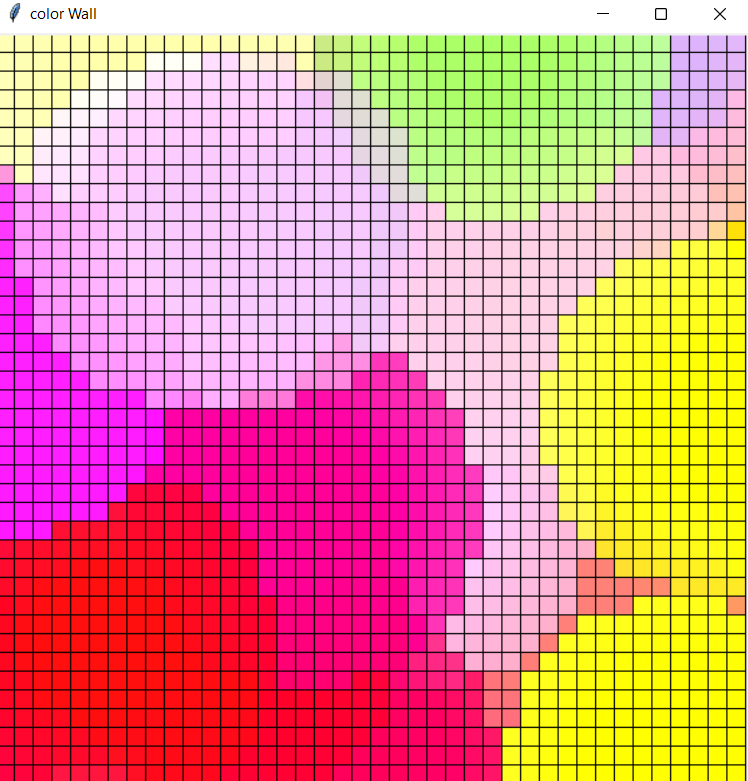
\includegraphics[scale=0.8]{images/image1.png}
To compare the BMU of two different countries which logically should be in different clusters, I chose USA and Pakistan. Pakistan having a much lower education rate than USA. To show which cluster their BMU resides in, I colored the BMU black. Repeatedly performing this provides similar results.\\
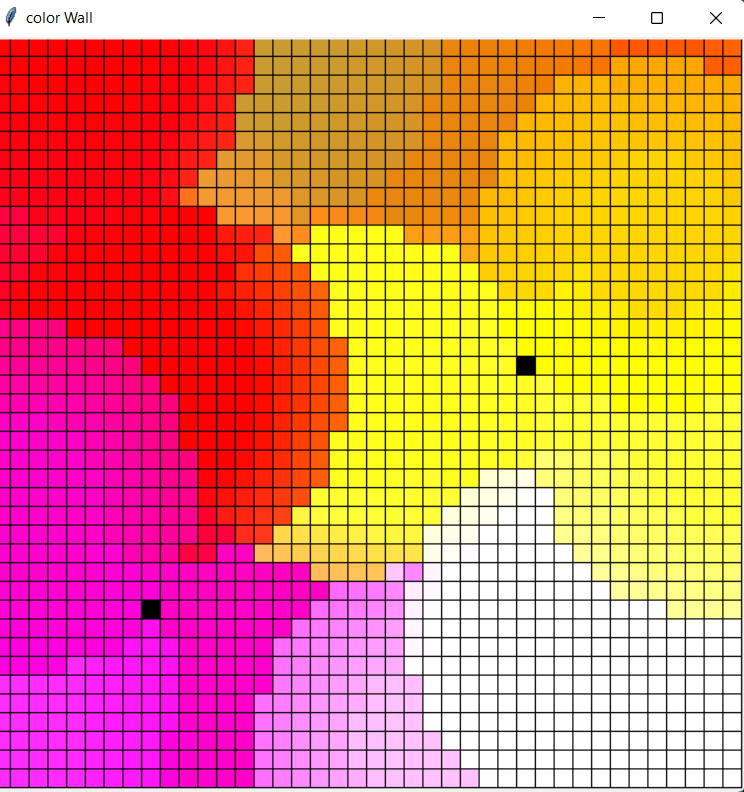
\includegraphics[scale=0.8]{images/image2.png}
\end{document}